

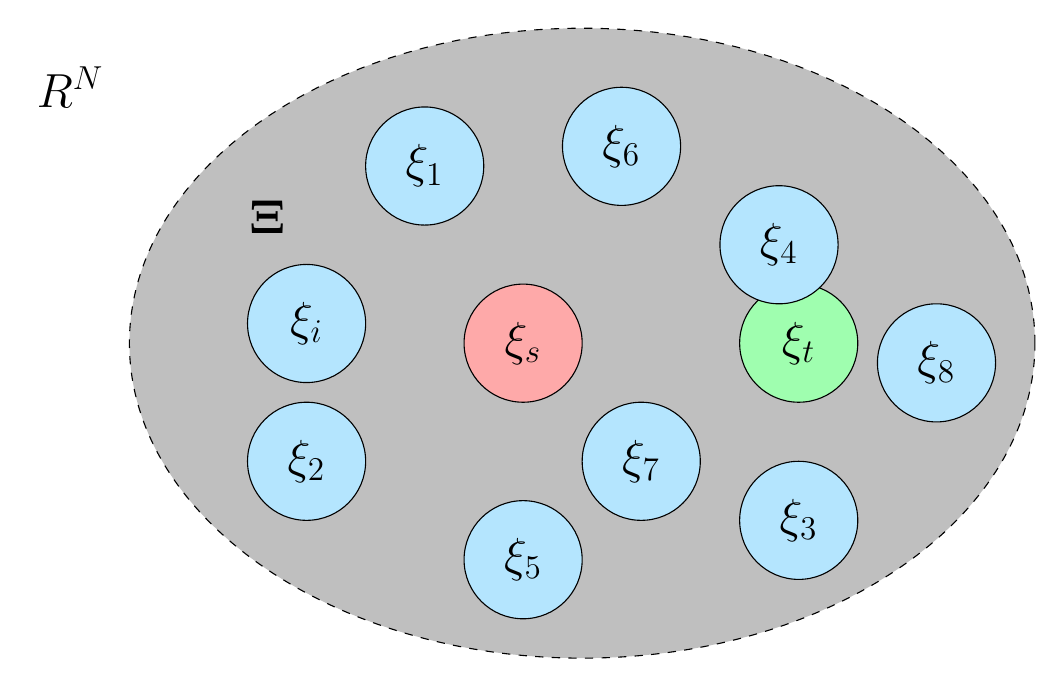
\begin{tikzpicture}[node distance=1cm, auto,]
\tikzstyle{every node}=[font=\LARGE]
\draw [ fill=gray!50, dashed] (8.25,7.75) ellipse (5.75cm and 4cm);
% \draw [dashed] (9.25 ,7.75) ellipse (3.25cm and 2cm);
\draw [ dashed] (14,11.75) ellipse (0cm and 0cm);
\draw [ dashed] (13,11.5) ellipse (0cm and 0cm);
\draw [ fill={rgb,255:red,180; green,229; blue,254} ] (4.75,8) circle (0.75cm) node {\LARGE $\xi_i$};
\draw [ fill={rgb,255:red,159; green,254; blue,175} ] (11,7.75) circle (0.75cm) node {\LARGE $\xi_t$};
\draw [ fill={rgb,255:red,180; green,229; blue,254} ] (6.25,10) circle (0.75cm) node {\LARGE $\xi_1$};
\draw [ fill={rgb,255:red,180; green,229; blue,254} ] (4.75,6.25) circle (0.75cm) node {\LARGE $\xi_2$};
% \draw [ fill={rgb,255:red,180; green,229; blue,254} ] (9.25,9) circle (0cm) node {\LARGE $\xi_3$};
% \draw [ fill={rgb,255:red,180; green,229; blue,254} ] (10,9) circle (0cm) node {\LARGE $\xi_4$};
\draw [ fill={rgb,255:red,180; green,229; blue,254} ] (11,5.5) circle (0.75cm) node {\LARGE $\xi_3$};
\draw [ fill={rgb,255:red,180; green,229; blue,254} ] (10.75,9) circle (0.75cm) node {\LARGE $\xi_4$};
\draw [ fill={rgb,255:red,180; green,229; blue,254} ] (7.5,5) circle (0.75cm) node {\LARGE $\xi_5$};
\draw [ fill={rgb,255:red,180; green,229; blue,254} ] (8.75,10.25) circle (0.75cm) node {\LARGE $\xi_6$};
\draw [ fill={rgb,255:red,180; green,229; blue,254} ] (9,6.25) circle (0.75cm) node {\LARGE $\xi_7$};
\draw [ fill={rgb,255:red,180; green,229; blue,254} ] (12.75,7.5) circle (0.75cm) node {\LARGE $\xi_8$};
\draw [ fill={rgb,255:red,254; green,169; blue,169} ] (7.5,7.75) circle (0.75cm) node {\LARGE $\xi_s$};
\node [font=\LARGE] at (4.25, 9.35) {$\mathbf{\Xi}$};
% \node [font=\LARGE] at (7.75, 9.25) {$\mathbf{\Theta}$};
\node [font=\LARGE] at (1.75, 11) {$\mathbb{R^N}$};


    
\end{tikzpicture}
